\documentclass[a4paper,14pt]{extarticle}

\def\labauthors{Сарафанов Ф.Г., Платонова М.В.}
\def\labgroup{440}
\def\labnumber{1}
\def\labstartdate{3 декабря}
\def\labtheme{Оценивание параметров  \\[0.2em] случайного процесса}
\def\shortlabtheme{Параметры случайного процесса}

%!TEX root = ../fet.tex
\usepackage{cmap}
\usepackage[T2A]{fontenc}
\usepackage[utf8x]{inputenc}
\usepackage[english, russian]{babel}

\usepackage{misccorr} % в заголовках появляется точка, но при ссылке на них ее нет
\usepackage{amssymb,amsfonts,amsmath,amsthm}  
\usepackage{indentfirst}
\usepackage[usenames,dvipsnames]{color} 
\usepackage[unicode,hidelinks]{hyperref}
% \hypersetup{%
%     pdfborder = {0 0 0}
% }

\usepackage{makecell,multirow} 
\usepackage{ulem}
\usepackage{graphicx,wrapfig}
\graphicspath{{img/}}
\usepackage{geometry}
\geometry{left=2cm,right=2cm,top=3cm,bottom=3cm,bindingoffset=0cm,headheight=15pt}
\usepackage{fancyhdr} 
\linespread{1.05} 
\frenchspacing 
\renewcommand{\labelenumii}{\theenumii)} 
\newcommand{\mean}[1]{\langle#1\rangle}
% \usepackage{caption}
%%%%%%%%%%%%%%%%%%%%%%%%%%%%%%%%%%%%%%%%%%%%%%%%%%%%%%%%%%%%%%%%%%%%%%%%%%%%%%%
%%%%%%%%%%%%%%%%%%%%%%%%%%%%%%%%%%%%%%%%%%%%%%%%%%%%%%%%%%%%%%%%%%%%%%%%%%%%%%%



%%%%%%%%%%%%%%%%%%%%%%%%%%%%%%%%%%%%%%%%%%%%%%%%%%%%%%%%%%%%%%%%%%%%%%%%%%%%%%%
	%применим колонтитул к стилю страницы
\pagestyle{fancy} 
	%очистим "шапку" страницы
\fancyhead{} 
	%слева сверху на четных и справа на нечетных
\fancyhead[L]{\labauthors} 
	%справа сверху на четных и слева на нечетных
\fancyhead[R]{\shortlabtheme} 
	%очистим "подвал" страницы
\fancyfoot{} 
	% номер страницы в нижнем колинтуле в центре
\fancyfoot[C]{\thepage} 
\renewcommand{\phi}{\varphi}
%%%%%%%%%%%%%%%%%%%%%%%%%%%%%%%%%%%%%%%%%%%%%%%%%%%%%%%%%%%%%%%%%%%%%%%%%%%%%%%

\usepackage{float}
\usepackage[mode=buildnew]{standalone}
\usepackage{tikz} 
% \usepackage{subcaption}
\usepackage{csvsimple}
\usetikzlibrary{scopes}
\usetikzlibrary{%
     decorations.pathreplacing,%
     decorations.pathmorphing,%
    patterns,%
    calc,%
    scopes,%
    arrows,%
    % arrows.spaced,%
}
\makeatletter
\newif\if@gather@prefix 
\preto\place@tag@gather{% 
  \if@gather@prefix\iftagsleft@ 
    \kern-\gdisplaywidth@ 
    \rlap{\gather@prefix}% 
    \kern\gdisplaywidth@ 
  \fi\fi 
} 
\appto\place@tag@gather{% 
  \if@gather@prefix\iftagsleft@\else 
    \kern-\displaywidth 
    \rlap{\gather@prefix}% 
    \kern\displaywidth 
  \fi\fi 
  \global\@gather@prefixfalse 
} 
\preto\place@tag{% 
  \if@gather@prefix\iftagsleft@ 
    \kern-\gdisplaywidth@ 
    \rlap{\gather@prefix}% 
    \kern\displaywidth@ 
  \fi\fi 
} 
\appto\place@tag{% 
  \if@gather@prefix\iftagsleft@\else 
    \kern-\displaywidth 
    \rlap{\gather@prefix}% 
    \kern\displaywidth 
  \fi\fi 
  \global\@gather@prefixfalse 
} 
\newcommand*{\beforetext}[1]{% 
  \ifmeasuring@\else
  \gdef\gather@prefix{#1}% 
  \global\@gather@prefixtrue 
  \fi
} 
\makeatother

\usepackage{booktabs}
\usepackage{pgfplots, pgfplotstable}

\usepackage[outline]{contour}
\usepackage{tocloft}
\renewcommand{\cftsecleader}{\cftdotfill{\cftdotsep}} % for parts
% \renewcommand{\cftchapleader}{\cftdotfill{\cftdotsep}} % for chapters
\usepackage{pgfplots,pgfplotstable,booktabs,colortbl}
\pgfplotsset{compat=newest}
\usepackage{physics}
\usepackage{mathtools}
\mathtoolsset{showonlyrefs=true}
\newcommand\Smat{\hat { \mathbf { S } }}

\newcommand*\dotvec[1][1,1]{\crossproducttemp#1\relax}
\def\crossproducttemp#1,#2\relax{{\qty[\vec{#1}\times\vec{#2}\,]}}

\newcommand*\prodvec[1][1,1]{\crossproducttempa#1\relax}
\def\crossproducttempa#1,#2\relax{{\qty[{#1}\times{#2}\,]}}

% \def\E{\mathscr{E}_H}
\def\Rdim{\,\frac{\text{м}^3}{\text{А} \cdot \text{с}}}

\renewcommand{\vec}{\mathbf} % for parts
\newcommand{\D}[1]{D\qty[#1]}

\begin{document}
%!TEX root = ../fet.tex
\begin{titlepage}
\begin{center}
% \vspace{-3em}
{\small\textsc{Нижегородский государственный университет имени Н.\,И. Лобачевского}}
\vskip 2pt \hrule \vskip 3pt
{\small\textsc{Радиофизический факультет}}

\vfill


{{\large Отчет по лабораторной работе №\labnumber}\vskip 12pt {\LARGE \bfseries \labtheme}}

	
\vspace{2cm}
{\large Работу выполнили студенты \\[-0.25em] \labgroup\  группы радиофизического факультата \\[0.5em] {\Large \bfseries \labauthors}}

% \vspace{0.5cm}
% {e-mail: sfg180@yandex.ru}

% \vspace{2cm}

\end{center}

\vfill
	
% \begin{flushright}
% 	{Выполнили студенты 430 группы\\ \labauthor}%\vskip 12pt Принял:\\ Менсов С.\,Н.}
% \end{flushright}
	
% \vfill
	
\begin{center}
	{Нижний Новгород, \labstartdate\ -- \today}
\end{center}

\end{titlepage}

\tableofcontents
\newpage



\addcontentsline{toc}{section}{Введение}
\section*{Введение}
% \vspace{-0.5em}
В настоящей работе изучаются вопросы, связанные с оценкой параметров случайных процессов, на примере оценки среднего значения (матожидания) случайного процесса.
% \vspace{-0.5em}
\newpage


% \paragraph{Установка с стержнями.} При оценке того или иного параметра случайного процесса следует:
% \begin{enumerate}
%     \item Выбрать алгоритм оценки параметра (записать формулу, которая показывает, какие действия нужно производить с числами $x_{1},x_{2},\dots,x_n$ -- результатами измерений), чтобы получить число, принимаемое нами за оценку интересующего нас параметра.
%     \item Исследовать выбранный алгоритм на предмет качества оценок. Качество оценки характеризуют ее \textbf{несмещенность}, \textbf{состоятельность} и \textbf{эффективность}:
%     \begin{enumerate}
%         \item Оценка называется \textbf{несмещенной}, если среднее статистическое её равно оцениваемой величине:  $\mean{\tilde a} = a$, где $a$ -- измеряемый параметр случайного процесса,  - его оценка\footnote{Оценка неизвестного параметра $a$ одним числом называется точечной}. Несмещенность оценки эквивалентна отсутствию систематической ошибки при измерении как в сторону ее завышения, так и в сторону ее занижения.
%     \item Оценка называется состоятельной, если при неограниченном росте объёма экспериментального материала дисперсия оценки стремится к нулю. При этом вероятность сколь угодно малых отклонений оценки от оцениваемой величины тоже стремится к нулю. Таким образом, если оценка состоятельна, то можно быть уверенным, что величина ошибки измерения не превосходит допустимую при достаточно большом, но ограниченном объеме статистического материала (т.е. достаточно большом времени измерения).
%     \item Если при измерении одной и той же характеристики случайного процесса можно пользоваться различными оценками, то эффективной называют оценку с наименьшей дисперсией. На практике не всегда удаётся удовлетворить всем этим требованиям. Например, может оказаться, что эффективная оценка существует, но формулы для её вычисления слишком сложны. Тогда приходится довольствоваться другой оценкой с несколько большей дисперсией. Иногда, в целях упрощения расчетов, применяются смещенные оценки. Но всегда выбору оценки должно предшествовать критическое изучение ее свойств.
%     \end{enumerate}
% \item Определить погрешность оценки параметра. 
% \end{enumerate}
% \section{Алгоритм оценки среднего значения}%
% \label{sec:algoritm_otsenki_srednego_znacheniia}
% Пусть мы имеем дело со случайной величиной $X$ и хотим найти её математическое ожидание.
% Алгоритм оценки среднего значения выбирается в виде:
% \begin{equation}
%     \label{eq:1.1}
%     \tilde x = \frac{1}{n} \sum\limits_{i=1}^{n} x_i \text{ для случайной величины)},
% \end{equation}
% где $x_i,~x_k$ -- результаты независимых измерений случайной величины;
% \begin{equation}
%     \label{eq:1.2}
%     \tilde x = \frac{1}{n} \sum\limits_{i=1}^{n} x_i(t_i) \text{ (для случайного процесса)},
% \end{equation}
% где $x_i(t_i)$ -- дискретные выборки значений процесса $x(t)$, взятые в дискретные,
% равноотстоящие на величину $\Delta t$, моменты времени ($\Delta t = t_{i+1}-t_i$ ).
% Этот алгоритм оценки естественен, поскольку известно, что $\frac{1}{n} \sum\limits_{i=1}^{n} x_i$-- среднеарифметическое $n$ независимых измерений случайной
% величины -- сходится по вероятности к среднему значению $\mean{x}^2$ (математическому
% ожиданию) при $n \to \infty $.

% Нетрудно показать, что оценки среднего \eqref{eq:1.1}, \eqref{eq:1.2}  являются
% \textbf{несмещенными} (т.е. не содержат систематической ошибки). Действительно, проводя
% статистическое усреднение левых и правых частей и учитывая эргодичность изучаемого
% случайного процесса, получаем $\mean{\tilde x} = \mean{x}$, т.е. статистическое среднее оценок равно среднему
% статистическому самого процесса.

% При получении оценки среднего значения стационарного эргодического процесса согласно 
% \eqref{eq:1.2}, усредняются дискретные выборочные значения процесса, отстоящие во времени 
% на $\Delta t$. Возникает закономерный вопрос, не проигрываем ли мы в чем то существенном,
% не используя информацию о процессе, заключающуюся в промежуточных значениях процесса,
% лежащих между дискретными отсчетами. Может быть, оценка среднего существенно улучшится,
% если взять ее в виде непрерывного усреднения реализации процесса на некотором временном 
% интервале, длительностью $T$, примыкающем к текущему моменту времени $t$:
% \begin{equation}
%     \label{eq:1.3}
%     \tilde x(t) = \frac{1}{T} \int\limits_{t-T}^{t} x(\tilde t) \dd{\tilde t} 
% \end{equation}

% В связи с тем, что при использовании численных методов сам интеграл в \eqref{eq:1.3}
% вычисляется приближенно через значения подынтегральной функции в отдельных дискретных точках. Оценку 
% \eqref{eq:1.3}  можно рассматривать как частный случай оценки \eqref{eq:1.2},
% если отсчеты берутся достаточно часто (если интервал между отсчетами существенно меньше 
% времени корреляции процесса $\Delta t \ll \tau_{\text{кор}}$). Тем не менее, имеет смысл
% рассмотреть аналитически [1] оценку среднего в виде (1.3) и убедиться в том, что величина
% погрешности оценки определяется лишь числом некоррелированных отсчетов содержащихся в 
% интервале усреднения $T$.
% Другими словами, если в оценке \eqref{eq:1.1}  взято $n$ некоррелированных отсчетов, а в
% оценке \eqref{eq:1.3}  интервал усреднения $T$ выбран равным $T = n \tau_{\text{кор}}$,
% оценки \eqref{eq:1.1}  и \eqref{eq:1.3}  оказываются эквивалентными по точности при $n\gg 1$. Следует проследить за выполнением этого утверждения при выполнении заданий №3,5.

% \section{Погрешность оценки}%
% \label{sec:pogreshnost_otsenki}
% На практике важно не просто получить оценку параметра, но и оценить, как близко значение оценки к истинному значению параметра. Другими словами, необходимо оценить погрешность оценки. Поскольку конкретное значение оценки параметра случайно (оно определяется конкретной выборкой $x_{1},x_{2},\dots,x_n$), то и ошибка конкретной оценки тоже случайна. Поэтому при рассмотрении погрешности оценки имеется в виду рассмотреть ее поведение на ансамбле независимых замеров оценки.

% За погрешность оценки принимаем среднеквадратическое отклонение оценки от среднего
% значения (корень квадратный из дисперсии оценки), т.е.
% \begin{equation}
%     \label{eq:2.1}
%     \sigma_{\tilde x} = \sqrt{ D\qty[\tilde x]} = \sqrt{ \mean{(\tilde x - \mean{x})^2} }
% \end{equation}
% или средний квадрат отклонения от истинного среднего. С.К.О. оценки показывают в каком интервале
% лежат оценки среднего.

% В предельном случае при $n=1$, (производится \textbf{однократный отсчёт}), и результат $x_{1}$ принимается за оценку среднего), ошибка конкретной оценки  $(x_{1}-\mean{x})$ естественно будет случайной,
% а погрешность оценки:
% \begin{equation}
%     \label{eq:2.2}
%     \sqrt{ \mean{ \qty( x_{1} - \mean{x} )^2 } } = \sqrt{D\qty[x]} = \sigma_x
% \end{equation}

% Из \eqref{eq:2.2} видно, что мерой погрешности оценки при $n=1$ является 
% среднеквадратическое отклонение (СКО) исследуемой случайной величины (корень квадратный из дисперсии
% исходного процесса в случае \eqref{eq:1.1} ).

% Известно, что при усреднении <<$n$>> независимых одинаково распределенных
% слагаемых дисперсия уменьшается в $n$ раз
% \begin{equation}
%     \label{eq:2.3}
%     \sigma_{\tilde x} = \sqrt{ \frac{D\qty[x] }{n}}
% \end{equation}

% Если же оценивается среднее значение эргодического процесса, согласно алгоритму
% \eqref{eq:1.2}, дисперсию оценки $D\qty[\tilde x] = \mean{ \qty( \tilde x - \mean{x} )^2 }$
% можно записать [1] в виде
% \begin{equation}
%     \label{eq:2.4}
%     D\qty[\tilde x] = \frac{\D{x}}{n} + \frac{1}{n^2} \sum\limits_{i=1}^{n} \sum\limits_{j\neq i}^{n} B_x(t_i - t_j),
% \end{equation}
% где $B_x(t_i - t_j) = \mean{ (x_i - \mean{x}) (x_i - \mean{x})  }$ -- функция
% ковариации процесса  $x(t)$, причем $\D{x}$ -- дисперсия процесса $x(t)$ -
% равна $\D{x}=B_x(0)$.

% При $n \to \infty$ дисперсия оценки стремится к нулю $\D{\tilde x} \to 0$, т.е.
% оценка является \textbf{состоятельной}.

% Из \eqref{eq:2.4} видно, что величина $\D{\tilde x}$ дисперсии оценки \eqref{eq:1.2} 
% существенно зависит от степени коррелированности отсчетов, а значит от того, насколько
% велик интервал между отсчетами $\Delta t$ по сравнению с $\tau_{\text{кор}}$ - временем
% корреляции процесса ( $t_{\text{кор}}$ -- эффективная протяженность $B_x(\tau)$ - 
% функции ковариации процесса $x(t)$ ).


% Здесь есть две предельные ситуации:
% \begin{enumerate}
%     \item Все $n$ отсчетов укладываются на времени, существенно меньшем времени корреляции
%         процесса ($n\cdot \Delta t \ll \tau_{\text{кор}}$), тогда дисперсия оценки равна
%         дисперсии исходного процесса $\D{\tilde x}= \D{x}$. В этом случае <<n>> отсчетов
%         по влиянию на точность оценки эквивалентны одному отсчету.
%     \item  Если же $\Delta t \geq \tau_{\text{кор}}$, то можно принять  и дисперсия оценки \eqref{eq:1.2} 
%         оказывается равной, т.е. дисперсия оценки аналогично \eqref{eq:2.3}  в <<n>> раз уменьшается по сравнению с дисперсией процесса, где <<n>> ‑ число некоррелированных отсчетов в оценке \eqref{eq:1.2} .

% Поведение СКО оценки при произвольных $\Delta t$ исследуется в заданиях №№ 3, 4.
% \end{enumerate}


% \section{Оценка среднего значения и погрешности оценки среднего при помощи спектральной 
% плотности мощности}%

% Как уже рассматривалось выше, если $x(t)$ -- случайный эргодический процесс, то среднее
% $\mean{x}$ может быть найдено путем усреднения по времени в виде \eqref{eq:1.3}.

% Корреляционная функция процесса $x(t)$ :
% \begin{equation}
%     \label{eq:}
%     K_x\qty[\tau] = B_x[\tau] + \mean{x}^2,
% \end{equation}
% а спектральная плотность мощности:
% \begin{equation}
%     \label{eq:}
%     S_x(\omega) = S_{x-\mean{x}}(\omega) + 2 \pi \delta(\omega) \mean{x}^2.
% \end{equation}
% Т.е. в случае ненулевого среднего значения в спектре случайного процесса наблюдается $\delta$ - 
% функция на нулевой частоте, а дисперсия представляет собой площадь под непрерывной частью спектра.

% Оценку среднего значения процесса в виде \eqref{eq:1.3}  можно рассматривать, как некоторый новый процесс,
% полученный из исходного путем линейного преобразования. В задании №5 рассматривается спектральная плотность мощности  оценки  в виде \eqref{eq:1.3} . Как найти по  погрешность оценки \eqref{eq:1.3}. Исследовать, как изменяется  с увеличением времени усреднения $T$, за счет чего при этом уменьшается погрешность оценки среднего.
% Для объяснения результатов этого задания, необходимо иметь в виду, что спектральная плотность мощности оценки среднего значения в виде \eqref{eq:1.3} , т.е. $S_{\tilde x}(\omega)$, связана со спектральной плотностью мощности исходного процесса $S_x(\omega)$  соотношением
% \begin{equation}
%     \label{eq:4.1}
%     S_{\tilde x}(2 \pi f) = S_x(2 \pi f) \abs{K(j 2 \pi f)}^2
% \end{equation}

% Коэффициент передачи  $K(j 2 \pi f)$ линейного преобразования \eqref{eq:1.3}  можно найти, как комплексную амплитуду выходного гармонического колебания, если же вместо входного 
% процесса  $\tilde x(t)$ в \eqref{eq:1.3}  подставить $e^{j 2 \pi f t}$ (гармоническое колебание единичной амплитуды и частоты $2 \pi f$). При этом окажется, что 
% \begin{equation}
%     \label{eq:4.2}
%     \abs{K(j_{2} \pi f)}^2 = \abs{\frac{\sin{\pi f T}}{\pi f T}}^2
% \end{equation}

% Из \eqref{eq:4.2}  видно, что усреднитель \eqref{eq:1.3} действует как фильтр,
% пропускающий спектральные составляющие в эффективной полосе $\Delta f_x = \frac{1}{2T}$,
% примыкающей к $f=0$. Постоянная составляющая, а также $S_{\tilde x}(0)$ спектральная плотность
% мозности процесса $\tilde x(t)$ на нулевой частоте, при этом остаются неизменными, т.к.
% $K(j 2 \pi f) \eval_{f=0}=1$. С увеличением $T$, уменьшается полоса пропускания этого фильтра,
% а значит и $\D{\tilde x}$ -- дисперсии оценки \eqref{eq:1.3},
% приближенно равная $\D{\tilde x}=S_{\tilde x}(0)\cdot \Delta f_{\tilde x} = S_{\tilde x}(0) \frac{1}{2T}$.

% При выполнении задания №5 следует убедиться, что $\D{\tilde x} = \frac{\D{x}}{T / \tau_{\text{кор}}}$, (при $T\gg \tau_{\text{кор}}$ ), т.е.
% погрешность оценки \eqref{eq:1.3} определяется только числом некоррелированных отсчетов,
% содержащихся в интервале усреднения $T$.

% В этом задании следует получить так же оценку среднего значения и оценить ее 
% погрешность непосредственно по спектральной плотности мощности процесса $\tilde x(t)$. 
% Эта оценка оказывается по существу эквивалентной оценке \eqref{eq:1.3}  при времени усреднения $T$,
% равном тому временному интервалу $T^*$, на котором мы находим Фурье-преобразование процесса 
% (в нашем случае $T^*=2048$); а ширина спектральной плотности мощности оценки, определяющая 
% ее дисперсию, обратна длине этого интервала и равна $1/2048$ (по существу это ширина 
% интервала частотного разрешения в спектре при выбранных параметрах Фурье-преобразования).

% \section{Доверительный интервал и доверительная вероятность}%
% \label{sec:doveritel_nyi_interval_i_doveritel_naia_veroiatnost_}
% Выше за количественную характеристику погрешности оценки среднего значения было взято СКО 
% оценки (корень квадратный из дисперсии оценки). Но в связи с тем, что оценка является 
% случайной величиной, определяемой случайными выборочными значениями $x_1,x_2,\dots,x_n$,
% на практике возможна реализация таких значений оценки, которые отличаются от истинного
% значения среднего больше, чем на величину СКО оценки. Как часто это может происходить, и
% какой должна быть выбрана длина интервала, характеризующего погрешность оценки, чтобы с
% достоверностью неизвестное среднее отстояло от случайной оценки не дальше, чем на величину 
% выбранного интервала? Сначала несколько слов о том, что значит с достоверностью? При какой 
% вероятности появление события его можно считать практически достоверным? Эта вероятность 
% определяется существом исходной задачи. В некоторых задачах это может быть $0.90$ или $0.95$; $0.99$ и т.д. Эту вероятность будем называть доверительной и обозначать $\beta$. 
% По этой вероятности выбирается $I_{\beta}$ величина интервала, называемого доверительным 
% (обычно его длина выражается в долях среднеквадратического значения оценки $I_{\beta}=t_{\beta} \sigma_{{\tilde x}}$). 
% Если отложить этот интервал вокруг случайного значения оценки, то он с доверительной 
% вероятностью $\beta$ накроет неизвестное среднее значение $\mean{x}$ (т.е. практически с достоверностью).

% Величина доверительного интервала выражается через плотность вероятностного распределения о
% оценки $W(\tilde x)$ и доверительную вероятность $\beta$ согласно соотношению:
% \begin{equation}
%     \label{eq:5.1}
%     P\qty(\abs{\mean{x}} - \tilde x \leq I_{\beta}) = \int\limits_{\mean{x}-I_{\beta}}^{\mean{x}+I_{\beta}}  W(\tilde x) \dd{\tilde x} = \beta
% \end{equation}

% В значительном ряде случаев принимается, что плотность вероятности оценки  $W(\tilde x)$ распределена по закону Гаусса (по закону Гаусса зачастую распределена и сама величина $X$,
% среднее значение которой оценивается, но если $X$ не имеет гауссова распределения, то 
% можно принять распределенной по закону Гаусса саму оценку $\tilde x$  при достаточно большом числе 
% усредняемых некоррелированных слагаемых в \eqref{eq:1.1}  в силу центральной предельной теоремы теории вероятностей).
% При небольших $n$ ($n\leq 15$ ) распределение оценки $\tilde x$ нельзя считать 
% Гауссовым даже в том случае, когда $X$ -- распределено по закону Гаусса, если 
% неизвестна дисперсия величины $X$ и она оценивается по тем же <<n>> отсчетам. 
% Подробнее об этом сказано в примечании к заданию №6. 
% В этом случае следует находить доверительный интервал для оценки, считая, что относительная величина оценки $\frac{\tilde x}{\sigma_{\tilde x}}$ распределена по
% закону Стьюдента с числом степеней свободы равным <<n-1>> (где $n$ -- число 
% усредняемых некоррелированных отсчетов в оценке \eqref{eq:1.1}  и, пользуясь соответствующими таблицами, имеющимися в справочной литературе).

% Вопросы, связанные с описание погрешности оценки через доверительный интервал и доверительную вероятность, рассматриваются в задани  №6.


















\section{Лабораторный эксперимент}
Для выполнения лабораторной работы использовалась вспомогательная программа, предоставляющая возможность сгенерировать гауссов шум с заданным временем корреляции $\tau_\text{корр}$, усреднить $M$ реализаций скользящим средним с регулируемыми шириной окна $N$, периодом дискретизации $\Delta t$.

Для сгенерированного сигнала программа позволяет рассчитать среднее значение, СКО и доверительный интервал, получить графики зависимостей СКО от параметров усреднения, графики реализаций и спектров, гистограммы оценок среднего значения.

\subsection{Реализации случайных процессов и их спектров}

Для иллюстрации случайных процессов были сгенерированы реализации дискретного гауссова шума для разных времен корреляции $\tau_\text{корр}$ (10,30,100) и построены графики как самих реализаций, так и их СПМ\footnote{СПМ -- здесь и далее -- спектральная плотность мощности}.

\begin{figure}[H]
    \centering
    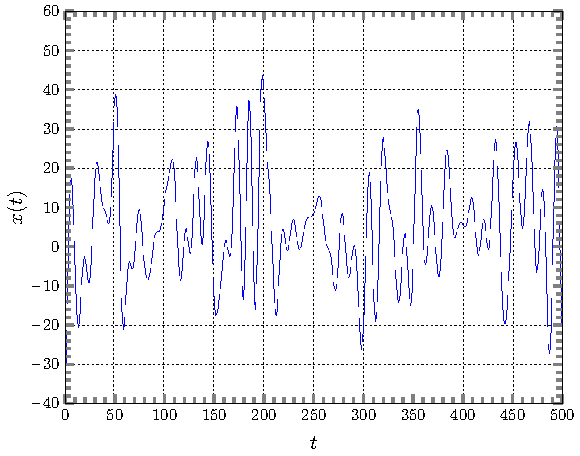
\includegraphics[width=0.7\linewidth]{fig/x_from_t_10.pdf}
    \vspace{-0.7em}
    \caption{Реализация случайного процесса с $\tau_\text{корр}=10$}
    \label{fig:t10}
\end{figure}

\begin{figure}[H]
    \centering
    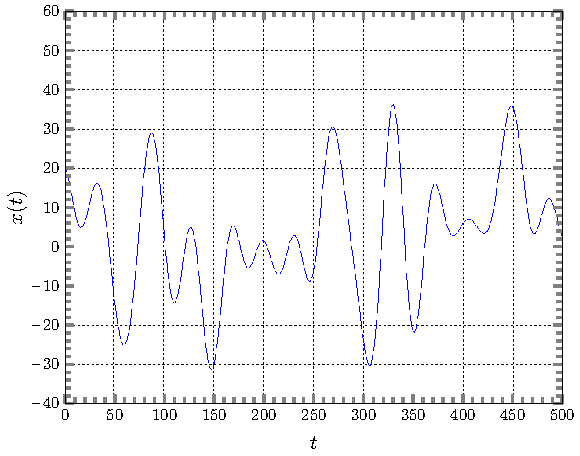
\includegraphics[width=0.7\linewidth]{fig/x_from_t_30.pdf}
    \vspace{-0.7em}
    \caption{Реализация случайного процесса с $\tau_\text{корр}=30$}
    \label{fig:t30}
\end{figure}


\begin{figure}[H]
    \centering
    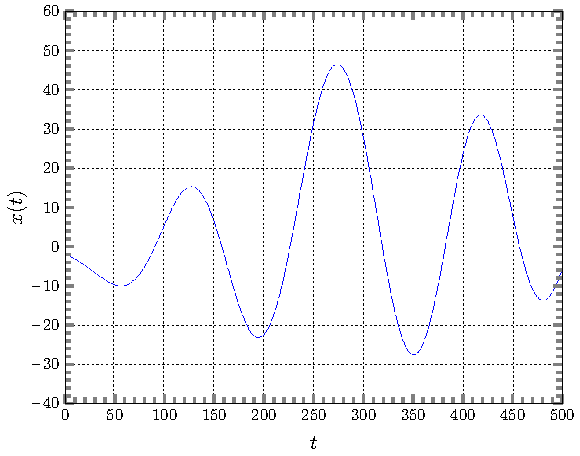
\includegraphics[width=0.7\linewidth]{fig/x_from_t_100.pdf}
    \vspace{-0.7em}
    \caption{Реализация случайного процесса с $\tau_\text{корр}=100$}
    \label{fig:t100}
\end{figure}

\begin{figure}[H]
    \centering
    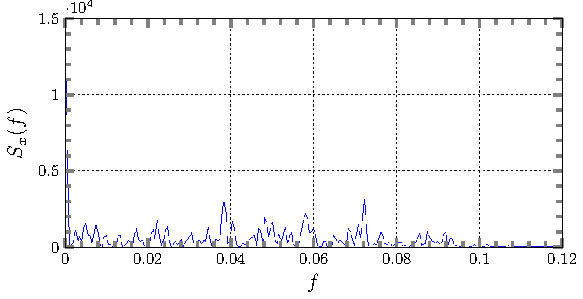
\includegraphics[width=0.7\linewidth]{fig/S_from_f_10.pdf}
    \vspace{-0.7em}
    \caption{СПМ случайного процесса с $\tau_\text{корр}=10$}
    \label{fig:s10}
\end{figure}

\begin{figure}[H]
    \centering
    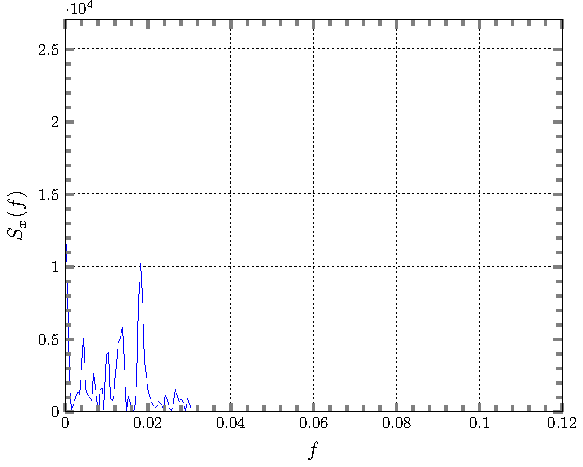
\includegraphics[width=0.7\linewidth]{fig/S_from_f_30.pdf}
    \vspace{-0.7em}
    \caption{СПМ случайного процесса с $\tau_\text{корр}=30$}
    \label{fig:s30}
\end{figure}

\begin{figure}[H]
    \centering
    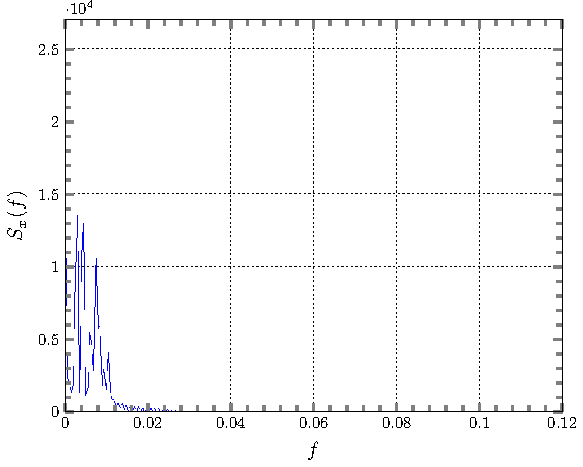
\includegraphics[width=0.7\linewidth]{fig/S_from_f_100.pdf}
    \vspace{-0.7em}
    \caption{СПМ случайного процесса с $\tau_\text{корр}=100$}
    \label{fig:s100}
\end{figure}

На графиках СПМ (см. рис. \ref{fig:s10}, \ref{fig:s30}, \ref{fig:s100}) хорошо видно, что ширина спектра обратно пропорциональна времени корреляции\footnote{Время корреляции $\tau_\text{кор}$  -- это время, при котором функция корреляции $\mathrm{B}[\tau]$ спадает в $e$ раз}. Это объясняется тем, что при больших временах корреляции два близких во времени отсчета сигнала отличаются слабо и сигнал меняется медленно, следовательно, имеет меньшую ширину спектра. Для малых времен применимы аналогичные рассуждения.


\subsection{Зависимость $\mean{x}$ от ширины окна усреднения $N$}
При заданных времени корреляции генерируемого сигнала $t_\text{корр}=10$, числе реализаций $M=128$, времени дискретизации $\Delta t=1$, ширине окна усреднения (количество усредняемых отсчетов) $N=1$ с помощью программы определены оценки среднего и СКО:
\begin{equation}
    \mean{x}=4.68, \quad \sigma_x = 14.74
\end{equation}

Также при времени корреляции генерируемого сигнала $t_\text{корр}=10$, числе реализаций $M=8$, времени дискретизации $\Delta t=1$ определена зависимость оценки от ширины окна усреднения ($N$):
\begin{figure}[H]
    \centering
    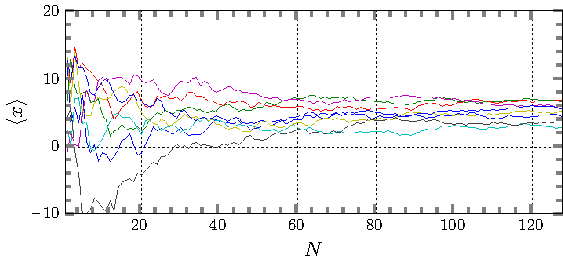
\includegraphics[width=0.8\textwidth]{fig/mean_from_N}
    \caption{Оценка среднего в зависимости от числа усредняемых отсчетов}
    \label{fig:mean_from_n}
\end{figure}

Разброс среднего от вертикали определяет собой \textit{дисперсию}. Разброс при $N=1$ составляет $\delta \mean{x}\approx15$, при $N=40$ соответственно $\delta \mean{x}\approx8$, и при $N=128$, наконец, $\delta \mean{x}\approx5$.





\subsection{Зависимость $\sigma_x$ от ширины окна усреднения $N$}
При заданных времени корреляции генерируемого сигнала $t_\text{корр}=10$, числе реализаций $M=256$, найдена серия зависимостей зависимость оценки от ширины окна усреднения ($N$) при разных временах дискретизации:
\begin{figure}[H]
    \centering
    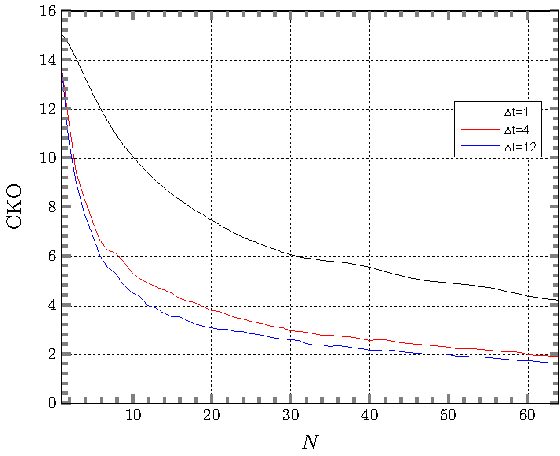
\includegraphics[width=0.8\textwidth]{fig/sko_t10.pdf}
    \caption{Зависимость СКО от числа усредняемых отсчетов}
    \label{fig:sko_from_n_t10}
\end{figure}
На графике видно, что с ростом времени корреляции СКО уменьшается. Действительно, так как оценка среднего совпадет\footnotemark{} с истинным значением при $T \to \infty$, то увеличивая время корреляции, мы приближаемся к условию $T \to \infty$, а значит, уменьшаем СКО.
\footnotetext{
Оценка среднего случайного процесса определяется как
\begin{equation}
    \label{eq:}
    \tilde x(t) = \lim_{T \to \infty} \int\limits_{0}^{T = n\cdot \tau_{\text{кор}}}  x(t) \dd{t}
\end{equation}}



\newpage
Аналогичная серия при тех же параметрах, но времени корреляции 100:
\begin{figure}[H]
    \centering
    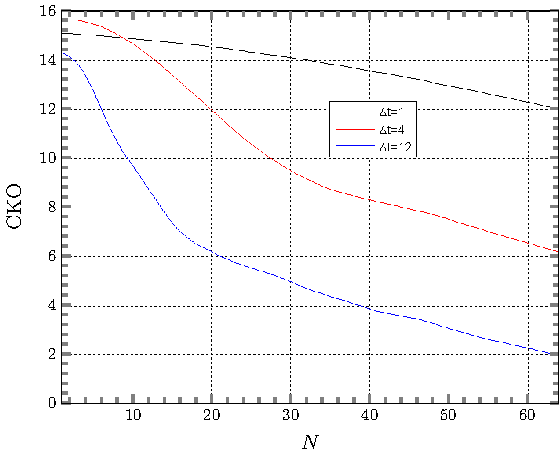
\includegraphics[width=0.8\textwidth]{fig/sko_t100.pdf}
    \caption{Зависимость СКО от числа усредняемых отсчетов}
    \label{fig:sko_from_n_t100}
\end{figure}
Заметим, что можно оценить время корреляции процесса по графику. Так как в случае $\Delta t \cdot N^* \ge \tau_\text{кор}$ 
\begin{equation}
    D[\tilde{x}] = \frac{D[x]}{N},
\end{equation}
то график $\sigma_x(N)$ после $\Delta t \cdot N^* = \tau_\text{кор}$ будет вести себя как гипербола. По точке перехода графика в гиперболу $N^*$ можно определить $\tau_\text{кор}$.

СКО оценки при $N=1$ определяется числом реализаций сигнала $M$. В таком случае для каждой реализации среднее значение - это значение единственного элемента в реализации. Другими словами, СКО оценки при $N=1$ определяется как дисперсия исходного процесса $D[x]$.



\subsection{Зависимость $\sigma_x$ от времени дискретизации $\Delta t$}

\begin{figure}[H]
    \centering
    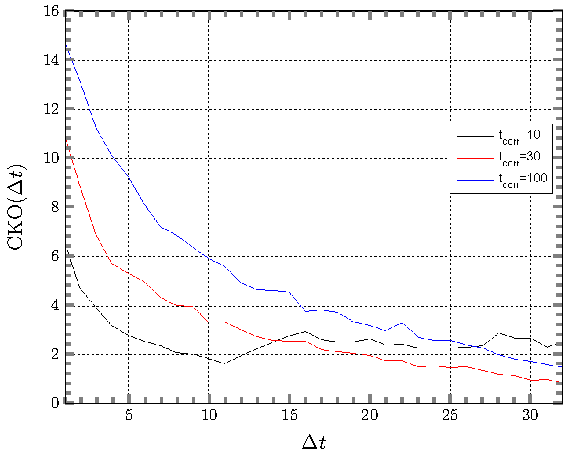
\includegraphics[width=0.7\linewidth]{fig/sko_n4.pdf}
    \vspace{-0.7em}
    \caption{$N=4$}
    \label{fig:sko_n4}
\end{figure}

\begin{figure}[H]
    \centering
    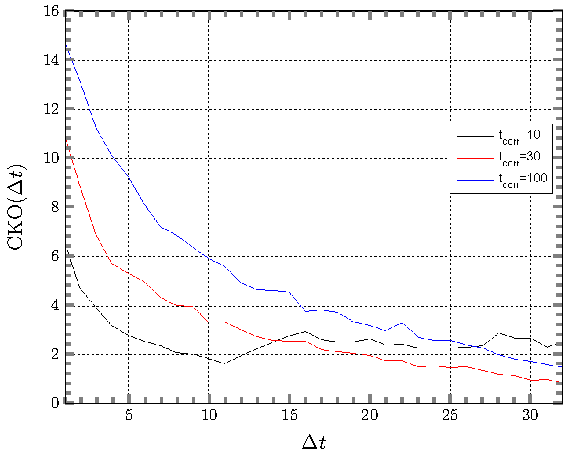
\includegraphics[width=0.7\linewidth]{fig/sko_n32.pdf}
    \vspace{-0.7em}
    \caption{$N=32$}
    \label{fig:sko_n32}
\end{figure}




\subsection{Определение $\mean{x}$ и $\sigma_x$ по  СПМ процесса}

\subsubsection{Параметры исходного процесса}

\begin{figure}[H]
    \centering
    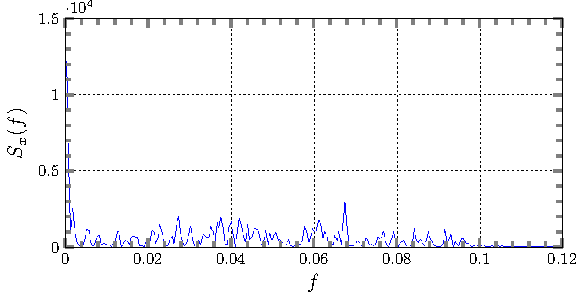
\includegraphics[width=0.7\linewidth]{fig/S_from_f_100_ex51}
    \vspace{-0.7em}
    \caption{$N=32$}
    \label{fig:sko_ex51}
\end{figure}

С помощью лабораторной программы строится график СПМ при $N=32$, $\tau_\text{корр}=10$. Из графика находится значение СПМ в нуле
\begin{equation}
    S_x(0) = 1.2\cdot 10^4
\end{equation}
Так как полная мощность в полосе $\Delta\omega = \frac{1}{2048}$ на нулевой частоте равна (с некоторой погрешностью) $\mean{x}^2 = S_x(0)\cdot \frac{1}{2048}$, то
\begin{equation}
    \mean{x}^2 = 1.2\cdot 10^4\cdot \frac{1}{2048} = 5.86
    \quad \Rightarrow \quad \mean{x}=2.42
\end{equation}
Из графика СПМ также можно найти дисперсию как произведение эффективной ширины спектра на эффективное значение СПМ:
\begin{equation}
    \mathrm{D}[\tilde{x}] = S_x(0)\cdot \Delta f_{\tilde{x}} =\frac{\mean{x}^2}{2} = 2.93 
    \quad \Rightarrow \quad
    \sigma_{\tilde{x}} = \sqrt{D[\tilde{x}]}\approx 1.71
\end{equation}


\subsubsection{Параметры усредненного процесса}

\begin{figure}[H]
    \centering
    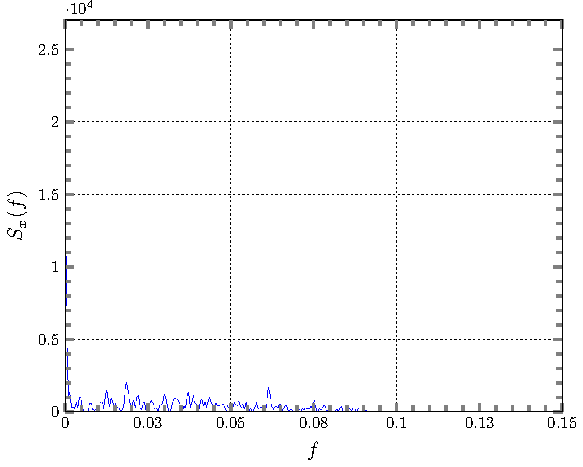
\includegraphics[width=0.7\linewidth]{fig/S_from_f_100_ex52_n4}
    \vspace{-0.7em}
    \caption{$N=4$}
    \label{fig:sko_ex52_n4}
\end{figure}

Аналогично операциям с исходным процессом, из графика при ширине окна усреднения $N=4$ находится величина СПМ в нуле, и простым расчетом находится среднее и дисперсия:
\begin{equation}
    S_x(0) = 1.25 \cdot 10^4
    \quad \Rightarrow \quad
    \mean{x}=2.43, \quad
    \sigma_{\tilde{x}} =  1.72
\end{equation}


\begin{figure}[H]
    \centering
    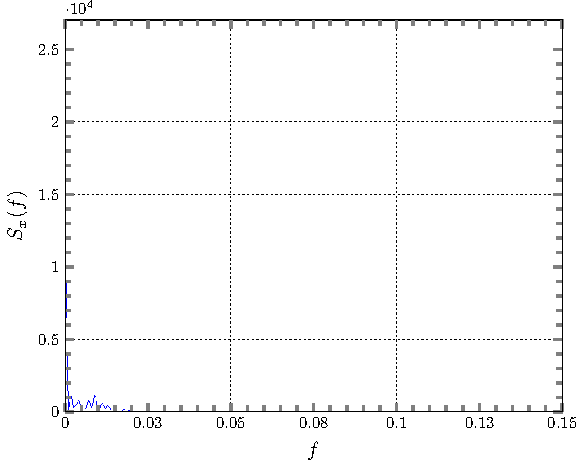
\includegraphics[width=0.7\linewidth]{fig/S_from_f_100_ex52_n32}
    \vspace{-0.7em}
    \caption{$N=32$}
    \label{fig:sko_ex52_n32}
\end{figure}

При усреднении с шириной окна $N=32$ получаются следующие параметры:
\begin{equation}
    S_x(0) = 1 \cdot 10^4
    \quad \Rightarrow \quad
    \mean{x}=1.99, \quad
    \sigma_{\tilde{x}} =  1.41
\end{equation}

\subsection{Доверительный интервал}
Можно исследовать влияние времени усреднения и доверительной вероятности на доверительный интервал. Для этого с помощью лабораторной программы построены гистограммы, иллюстрирующие распределение значений ансамбля из $M=256$ оценок среднего.

\subsubsection{Анализ гистограммы}
При заданных времени корреляции $\tau = 10$ и доверительной вероятности $\beta=0.95$, времени дискретизации $\Delta t=1$ получена серия гистограмм при разных ширинах окна усреднения $N=1, 4, 32$, отображенная на рисунках \ref{fig:g1}, \ref{fig:g4}, \ref{fig:g32}:
\vfill
\begin{figure}[H]
    \centering
    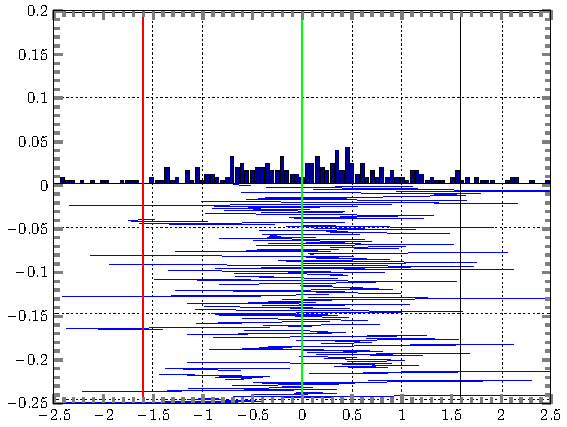
\includegraphics[width=0.75\linewidth]{fig/gist_n1}
    \vspace{-0.7em}
    \caption{$N=1$}
    \label{fig:g1}
\end{figure}
\vfill
\newpage
\begin{figure}[H]
    \centering
    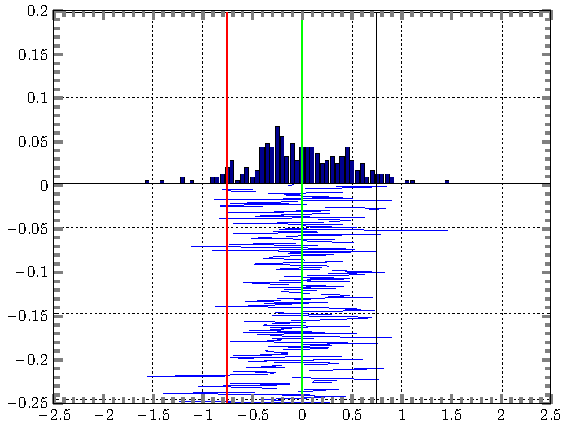
\includegraphics[width=0.75\linewidth]{fig/gist_n4}
    \vspace{-0.7em}
    \caption{$N=4$}
    \label{fig:g4}
\end{figure}
\begin{figure}[H]
    \centering
    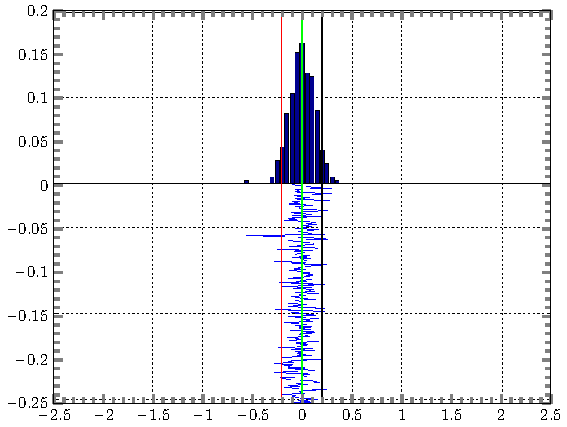
\includegraphics[width=0.75\linewidth]{fig/gist_n32}
    \vspace{-0.7em}
    \caption{$N=32$}
    \label{fig:g32}
\end{figure}
\subsubsection{Влияние доверительной вероятности}
При заданных времени корреляции $\tau = 10$, времени дискретизации $\Delta t=1$ получена серия $3\times3$ гистограмм при разных ширинах окна усреднения $N=1, 4, 32$ и разных доверительных вероятностях $\beta=0.8, 0.95, 0.98$:

\paragraph{Серия при $N=1$.} \hphantom{asasfsd}
\begin{figure}[H]
\begin{minipage}{0.3\linewidth}
    \centering
    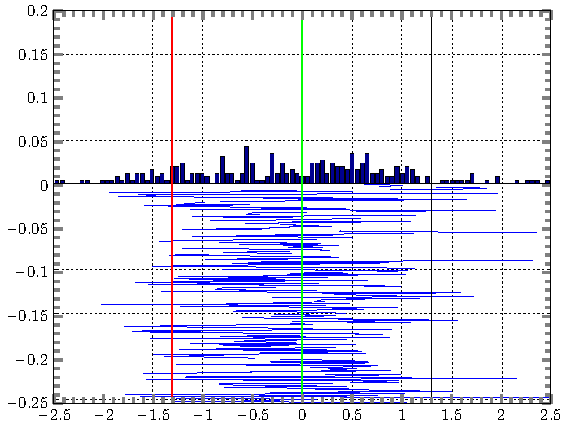
\includegraphics[width=\linewidth]{fig/gist_n1_b80.pdf}
    \vspace{-1em}
    \caption{$\beta =0.8$}
\end{minipage}
\begin{minipage}{0.3\linewidth}
    \centering
    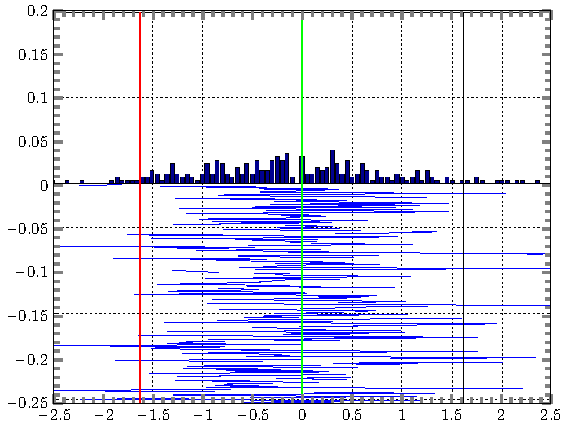
\includegraphics[width=\linewidth]{fig/gist_n1_b95.pdf}
    \vspace{-1em}
    \caption{$\beta =0.95$}
\end{minipage}
\begin{minipage}{0.3\linewidth}
    \centering
    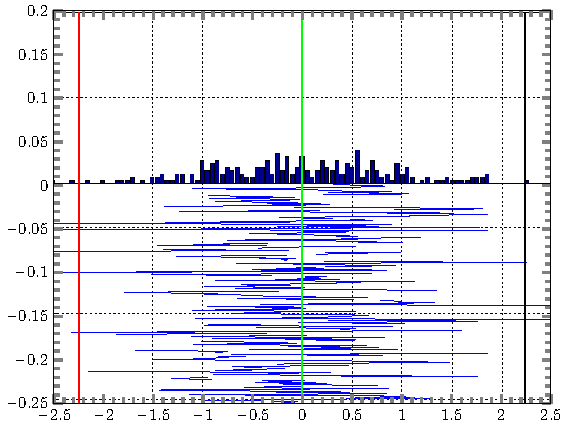
\includegraphics[width=\linewidth]{fig/gist_n1_b98.pdf}
    \vspace{-1em}
    \caption{$\beta =0.98$}
\end{minipage}
\end{figure}

\paragraph{Серия при $N=4$.} \hphantom{asasfsd}
\begin{figure}[H]
\begin{minipage}{0.3\linewidth}
    \centering
    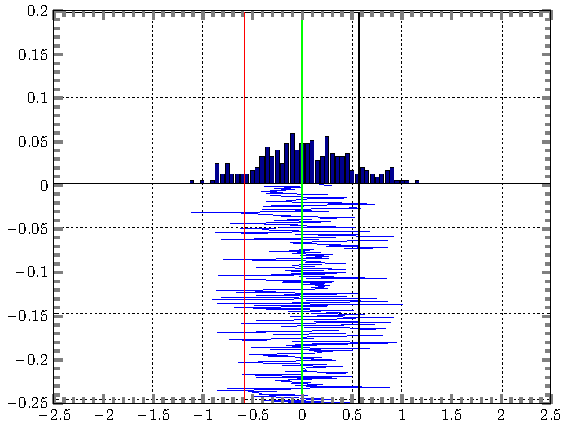
\includegraphics[width=\linewidth]{fig/gist_n4_b80.pdf}
    \vspace{-1em}
    \caption{$\beta =0.8$}
\end{minipage}
\begin{minipage}{0.3\linewidth}
    \centering
    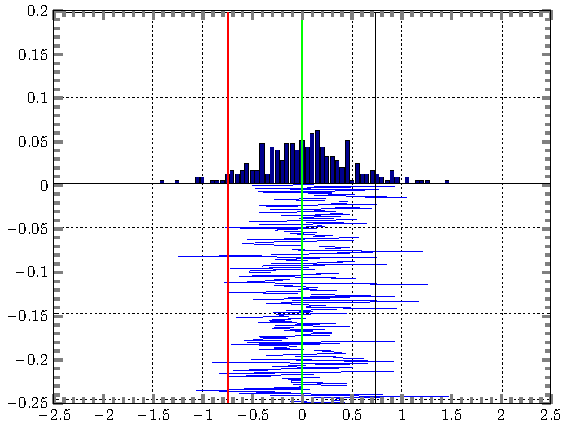
\includegraphics[width=\linewidth]{fig/gist_n4_b95.pdf}
    \vspace{-1em}
    \caption{$\beta =0.95$}
\end{minipage}
\begin{minipage}{0.3\linewidth}
    \centering
    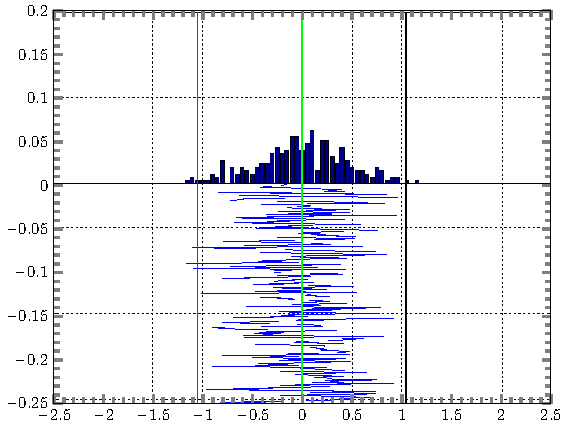
\includegraphics[width=\linewidth]{fig/gist_n4_b98.pdf}
    \vspace{-1em}
    \caption{$\beta =0.98$}
\end{minipage}
\end{figure}

\paragraph{Серия при $N=32$.} \hphantom{asasfsd}
\begin{figure}[H]
\begin{minipage}{0.3\linewidth}
    \centering
    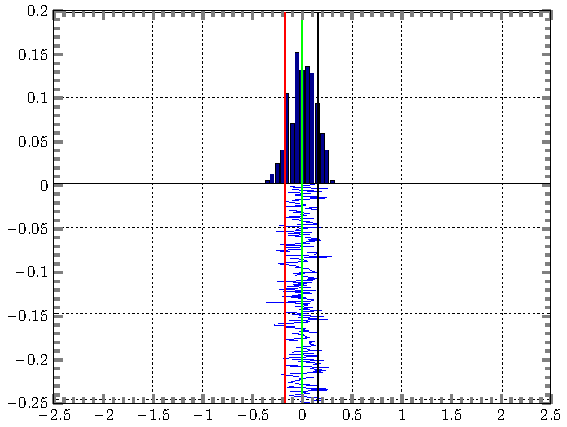
\includegraphics[width=\linewidth]{fig/gist_n32_b80.pdf}
    \vspace{-1em}
    \caption{$\beta =0.8$}
\end{minipage}
\begin{minipage}{0.3\linewidth}
    \centering
    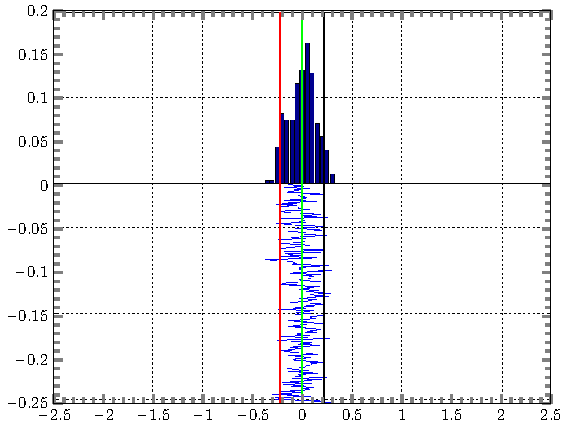
\includegraphics[width=\linewidth]{fig/gist_n32_b95.pdf}
    \vspace{-1em}
    \caption{$\beta =0.95$}
\end{minipage}
\begin{minipage}{0.3\linewidth}
    \centering
    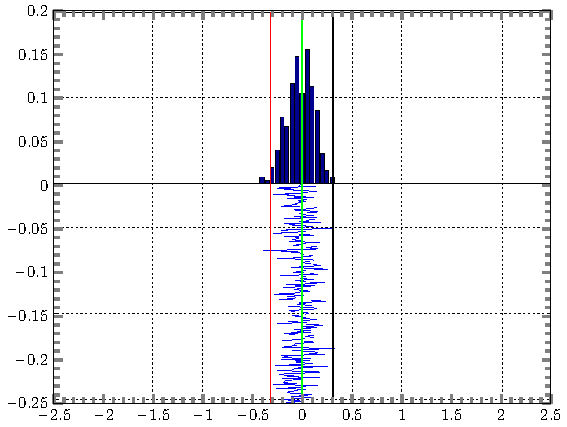
\includegraphics[width=\linewidth]{fig/gist_n32_b98.pdf}
    \vspace{-1em}
    \caption{$\beta =0.98$}
\end{minipage}
\end{figure}

По результатам серии измерений получена зависимость доверительного интервала $I$ от $\beta$ для разных значений $N$:
 \begin{figure}[H]
    \centering
    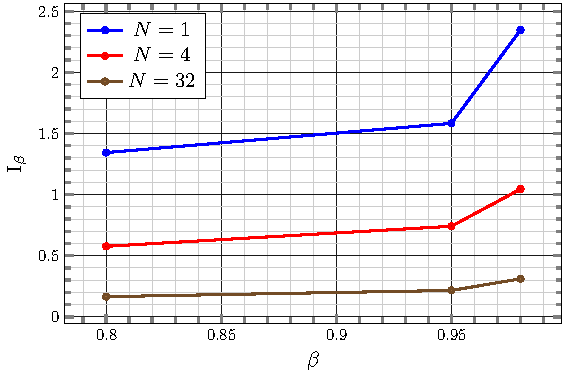
\includegraphics[width=0.8\linewidth]{fig/I_from_beta}
    \caption{График зависимости доверительного интервала $I$ от $\beta$}
\end{figure}
Из графика видно, что доверительный интервал растет с ростом $\beta$ и уменьшается при увеличении окна усреднения ($N\uparrow$).

\addcontentsline{toc}{section}{Заключение}
\section*{Заключение}

В результате выполнения данной работы мы изучили вёопросы, связанные с оценкой параметров случайных процессов на примере оценки их средних значений
В ходе выполнения 1-го задания мы установили, что вид реализации с ростом времени корреляции становится более плавным, а спектральная плотность мощности смещается ближе к нулевой частоте.
Так же мы установили, что значения разброса $\mean{x}$ по вертикали во втором задании больше значений $\mean{x}$ из задания 5 при любых $N$.
В результате выполнения 6-го задания было установлено, что доверительный интервал увеличивается при увеличении $\beta$ и уменьшается при увеличении количества отсчетов усреднения $N$.
\end{document}
